% BDE Guide --- Appendix: AU Tables
\chapter{Appendix: AU Summary Tables}
\label{ch:appendix-au}

This appendix gives the complete AU accounting for the single-degree BSc (Hons) in Computer Science (AY2024--25) in both official bucketings. The course list is identical; only the bucket labels differ by 1~AU at the College Core / BDE boundary. Degree Audit is authoritative for your cohort.

\section{Full 135~AU Map --- Both Bucketings}
\label{sec:au-buckets-table}

\begin{table}[h]
\centering
\small
\renewcommand{\arraystretch}{1.25}
\setlength{\tabcolsep}{3pt}\footnotesize\begin{tabular}{@{}p{3.6cm} c c p{6.0cm}@{}}
\toprule
Component & \multicolumn{2}{c}{AU} & Notes \\
 & Curriculum & PDF F-Core & \\
 & page & summary & \\
\midrule
University Core (ICC + CSL) & 17 & 17 & CC0001 (2) + CC0002 (2) + CC0003 (2) + CC0005 (3) + CC0006 (3) + CC0007 (3) + ML0004 (2) \\
College Core (Professional Series) & 16 & 15 (F-Core) & SC1003 (3) + HW0288 (2) + SC3920 (10) + 1~AU rounding/bridging \\
Programme Core & 47 & 47 (Core) & SC1004 (4), SC1005 (3), MH1812 (3), SC1006 (3), SC1007 (3), SC1008 (3), SC2000 (3), SC2002 (3), SC2001 (3), SC2005 (3), SC2203 (3), SC2006 (3), SC2008 (3), SC2207 (3), SC3099 (4) \\
Major Prescribed Electives (MPE) & 35 & 35 & FYP path: 9 courses $\times$ 3 + SC4079 (8) = 35; non-FYP: 12 $\times$ 3 = 36 (see text) \\
Broadening \& Deepening Electives (BDE) & 20 & 21 & Any approved NTU courses not counted elsewhere \\
\midrule
\textbf{Total} & \textbf{135} & \textbf{135} & Invariant; bucket labels shift by 1~AU at College/BDE boundary \\
\bottomrule
\end{tabular}
\caption{135~AU accounting: curriculum-page vs.\ PDF Foundational-Core bucketing. Both sum to 135; the 1~AU delta is a boundary shift, not extra workload.}
\label{tab:au-buckets}
\end{table}

\section{University Core Detail (17~AU)}
\label{sec:au-icc-detail}

\begin{table}[h]
\centering
\small
\renewcommand{\arraystretch}{1.22}
\begin{tabular}{@{}l c p{7.5cm}@{}}
\toprule
Course & AU & Title / purpose \\
\midrule
CC0001 & 2 & Inquiry \& Communication in an Interdisciplinary World \\
CC0002 & 2 & Navigating the Digital World \\
CC0003 & 2 & Ethics \& Civics in a Multicultural World \\
CC0005 & 3 & Healthy Living \& Wellbeing \\
CC0006 & 3 & Sustainability: Society, Economy \& Environment \\
CC0007 & 3 & Science \& Technology for Humanity \\
ML0004 & 2 & Career \& Innovative Enterprise for the Future World (CSL) \\
\midrule
Total & 17 & \\
\bottomrule
\end{tabular}
\end{table}

\section{College Core Detail (16~AU curriculum page / 15~AU PDF F-Core)}
\label{sec:au-college-detail}

\begin{table}[h]
\centering
\small
\renewcommand{\arraystretch}{1.22}
\begin{tabular}{@{}l c l p{5.0cm}@{}}
\toprule
Course & AU & When & Notes \\
\midrule
SC1003 & 3 & Y1 S1 & Intro to Computational Thinking \& Programming (NIL prereq) \\
HW0288 & 2 & Y3 & Engineering Communication (prereq CC0001 + Y3 standing) \\
SC3920 & 10 & Y3 S2 & Professional Internship (graded, Year~3 standing) \\
\midrule
\multicolumn{4}{@{}l}{\footnotesize Plus 1~AU bridging/rounding that appears under BDE in PDF summary.} \\
\bottomrule
\end{tabular}
\end{table}

\section{Programme Core Detail (47~AU)}
\label{sec:au-prog-detail}

\begin{table}[h]
\centering
\small
\renewcommand{\arraystretch}{1.22}
\begin{tabular}{@{}l c l p{4.2cm}@{}}
\toprule
Course & AU & Semester & Focus \\
\midrule
SC1004 & 4 & Y1 S1 & Linear Algebra for Computing \\
SC1005 & 3 & Y1 S1 & Digital Logic \\
MH1812 & 3 & Y1 S1 & Discrete Mathematics (cohort-dependent; SC1123/24 alt.) \\
SC1006 & 3 & Y1 S2 & Computer Organisation \& Architecture \\
SC1007 & 3 & Y1 S2 & Data Structures \& Algorithms \\
SC1008 & 3 & Y1 S2 & C/C++ Programming \\
SC2000 & 3 & Y1 S2 & Probability \& Statistics for Computing \\
SC2002 & 3 & Y1 S2 & Object-Oriented Design \& Programming \\
SC2001 & 3 & Y2 S1 & Algorithm Design \& Analysis \\
SC2005 & 3 & Y2 S1 & Operating Systems \\
SC2203 & 3 & Y2 S1 & Automata, Computability \& Complexity \\
SC2006 & 3 & Y2 S1 & Software Engineering \\
SC2008 & 3 & Y2 S1 & Computer Network \\
SC2207 & 3 & Y2 S2 & Introduction to Databases \\
SC3099 & 4 & Y3 S1 & Capstone Project (team, Programme Core) \\
\midrule
Total & 47 & & \\
\bottomrule
\end{tabular}
\end{table}

\section{MPE Detail (35~AU FYP path / 36~AU non-FYP)}
\label{sec:au-mpe-detail}

\begin{table}[h]
\centering
\small
\renewcommand{\arraystretch}{1.22}
\begin{tabular}{@{}p{5.0cm} c p{6.5cm}@{}}
\toprule
Path & AU & Composition \\
\midrule
FYP path (standard) & 35 & 9 MPE courses $\times$ 3~AU (any SC3xxx/4xxx, $\ge$4 at 4000-level) + SC4079 FYP (8~AU: 4+4 over Y4) \\
Non-FYP path & 36 & 12 MPE courses $\times$ 3~AU (any SC3xxx/4xxx, $\ge$4 at 4000-level); no FYP; Highest Distinction not eligible \\
\bottomrule
\end{tabular}
\end{table}

\noindent\textit{Note:} SC4079 is itself an MPE (not College Core). The FYP-or-3-MPE choice is governed by PDF Notes 2--3: Highest Distinction requires FYP. Confirm via Degree Audit; the non-FYP total of 136~AU may be adjusted via BDE/overload per audit.

\section{BDE Categories (20~AU / 21~AU)}
\label{sec:au-bde-detail}

\begin{table}[h]
\centering
\footnotesize
\renewcommand{\arraystretch}{1.22}
\setlength{\tabcolsep}{3pt}\footnotesize\begin{tabular}{@{}p{2.7cm} p{3.4cm} p{5.1cm}@{}}
\toprule
Category & Example codes & Notes \\
\midrule
Languages & LJ5001 (Japanese), LK5001 (Korean), LC5001 (Chinese), LF5001 (French) & 4~AU Level~1, 3~AU higher; placement test if prior knowledge \\
Business \& management & AB1601, AB1202, AC1103, BF1101, BM2501 & Check exclusions (e.g., AB1202 vs.\ SC2000) \\
HSS / Psychology & HP1000, HP8001, HH1001, HE9091 & No prerequisites for most; writing- or exam-heavy \\
Science / sustainability & CM8001, BS8003, ES9001 & Some have labs; not double-countable with ICC \\
Entrepreneurship & ET9131, ET9132, MN3001 & Project/pitch-heavy \\
Arts / design & HAxxxx, ADxxxx, HE-coded creative & Portfolio-based \\
\bottomrule
\end{tabular}
\end{table}

\begin{center}
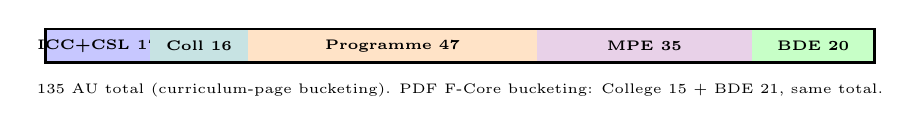
\begin{tikzpicture}[scale=0.78,every node/.style={font=\scriptsize}]
% Compact AU bar for appendix
\fill[blue!22] (0,0) rectangle (1.70,0.55); \node[font=\tiny\bfseries] at (0.85,0.27) {ICC+CSL 17};
\fill[teal!22] (1.70,0) rectangle (3.30,0.55); \node[font=\tiny\bfseries] at (2.50,0.27) {Coll 16};
\fill[orange!22] (3.30,0) rectangle (8.00,0.55); \node[font=\tiny\bfseries] at (5.65,0.27) {Programme 47};
\fill[violet!18] (8.00,0) rectangle (11.50,0.55); \node[font=\tiny\bfseries] at (9.75,0.27) {MPE 35};
\fill[green!22] (11.50,0) rectangle (13.50,0.55); \node[font=\tiny\bfseries] at (12.50,0.27) {BDE 20};
\draw[thick] (0,0) rectangle (13.50,0.55);
\node[font=\tiny,align=center] at (6.75,-0.45) {135~AU total (curriculum-page bucketing). PDF F-Core bucketing: College 15 + BDE 21, same total.};
\end{tikzpicture}
\end{center}

\section*{Verification Checklist for Your Cohort}
\begin{enumerate}[label=\arabic*.]
    \item Open Degree Audit (StudentLink $\to$ Academic $\to$ Degree Audit) and confirm each bucket shows Satisfied/In-Progress for your actual courses.
    \item For any BDE, verify in NTU Course Catalogue: AU, prerequisites, ``Mutually exclusive'' line, and MPE-list status for your cohort year.
    \item If Degree Audit and this guide disagree on AU bucketing, Degree Audit wins. If this guide and a senior disagree, Degree Audit wins.
\end{enumerate}

% End of Appendix
